\textbf{\textit{dio 1. revizije}}\\

\textit{Ovaj se projekt bavi razvojem programske podrške za web aplikaciju "TectonicHR". 
	Cilj aplikacije "TectonicHR" olakšano je prikupljanje podataka o intezitetu potresa te olakšani vizualni pristup informacijama. 
	Aplikacija je namijenjena znanstvenoj zajednici, ali i općoj populaciji. 
	Znanstvenoj zajednici, seizmolozima, bit će olakšan pristup informacijama i njihovo prikupljanje.  
	Opća populacija, građani, imat će mogućnost unosa novog potresa kojega su osjetili te pregled već zabilježenih potresa.   
	Prilikom otvaranja aplikacije građanima se nudi izbor odabira zadnjeg potresa u vidu datuma i vremena potresa te pretraživanje starih potresa. 
	Odabirom opcije "Stari potresi" pojavljuje se pregled preliminarne karte inteziteta potresa koja sadži interaktivnu kartu Hrvatske.
	Karta se prikazuje i pri opciji dodavanja informacija za zadnji potres. 
	Na karti je zvjezdicom označen epicentar te kružićem određene boje označen je intezitet potresa. (Hladnije plave nijanse označavaju slabiji intezitet, a tamnije crvene jači intezitet). 
	Ispod karte nalazi se tablica s podacima o zadnjem i starijim potresima. (KOJIM PODACIMA, DOGOVORI) 
	Ako se zadnji potres ne poklapa s opažanjima građana, preko opcije "Novi potres?" građanin može dodati novi potres koji je osjetio. 
	Kada građanin odluči dodati novi potres, obavezan je popuniti i predati upitnik. 
	Upitnik se sastoji od pitanja iz kojih znanstvenici mogu dobiti vrijedne informacije o tome kakvi su bili učinci potresa. 
	Građani moraju navesti kada i gdje se potres osjetio, gdje se osoba nalazila u to vrijeme, email te gdje se osoba nalazila u to vrijeme. 
	Nakon toga odgovara na pitanja o subjektivnom dojmu, kako je potres djelovao na osobu,  koliko se osjetilo. 
	Također, postavljaju se pitanja i o nastaloj šteti (oštećenim dimnnjacima i krovovima, ispucalim zidovima, srušenim građevinama).}

\begin{packed_item}
	\item \textit{potencijalna korist ovog projekta}
	\item \textit{postojeća slična rješenja (istražiti i ukratko opisati razlike u odnosu na zadani zadatak). Dodajte slike koja predočavaju slična rješenja.}
	\item \textit{skup korisnika koji bi mogao biti zainteresiran za ostvareno rješenje.}
	\item \textit{mogućnost prilagodbe rješenja }
	\item \textit{opseg projektnog zadatka}
	\item \textit{moguće nadogradnje projektnog zadatka}
\end{packed_item}

\textit{Za pomoć pogledati reference navedene u poglavlju „Popis literature“, a po potrebi konzultirati sadržaj na internetu koji nudi dobre smjernice u tom pogledu.}
\eject

Postoje tri vrste korisnika, a to su:
\begin{packed_item}
	\item anonimni korisnik (građanin)
	\item znanstvenik (seizmolog)
	\item administrator
\end{packed_item}

\underbar{Neregistriranom (anonimnom) korisniku} otvaranjem aplikacije prikazuje se izbornik u kojem može odabrati želi li pregledati aktualne potrese („Aktualni potresi“), pregledati arhivirane potrese („Arhivirani potresi“) ili ispuniti upitnik ako je osjetio novi potres („Novi potres?“). Klikom na „Aktualni potresi“ prikazuju mu se karta i popis potresa koje administrator još nije arhivirao. Anonimni korisnik može pretraživati te potrese i odabrati jedan potresa te za njega ispuniti upitnik. Na početnoj stranici, klikom na „Arhivirani potresi“ pokaže mu se karta i ispod nje popis potresa koje je administrator arhivirao. Prelaženjem kursorom preko oznake kojom je označen taj potres, prikazuju mu se osnovne informacije o potresu (datum, vrijeme, lokacija i intenzitet potresa).

\underbar{Seizmolog (znanstvenik)} se prijavljuje e-mailom i lozinkom. Seizmolog klikom na ikonu u kutu početnog zaslona odlazi na svoj profil gdje mu se omogućuje prikaz i promjena osobnih podataka (korisničko ime, ime, prezime, e-mail, lozinka). Ima sve mogućnosti kao i anonimni korisnik (ispunjavanje upitnika za novi potres, pregled karte i drugih podataka o aktualnim i arhiviranim potresima) uz još dodatnu ovlast preuzimanja podataka o potresima u .csv formatu.

\underbar{Administrator} ima najveće ovlasti. Početna stranica izgleda mu isto kao i seizmologu, ali mu se na stranici profila ispod njegovih podataka nalaze i dva gumba, „Novi upitnici“ i „Nove prijave“. Klikom na „Novi upitnici“ pregledava ispunjene upitnike koje još nije svrstao u nijedan potres. Upitnike može pridijeliti nekom već imenovanom potresu ili može stvoriti, imenovati i potvrditi novi potres te ih pridijeliti tom novostvorenom potresu. Klikom na „Nove prijave“ prikazuje mu se popis osoba koje žele biti registrirane kao znanstvenici. Odabirom jedne ili više prijava može ih registrirati. S početne stranice može pristupiti stranici aktualnih potresa. Na toj stranici može odabrati jedan ili više potres te ih arhivirati. Na stranici arhiviranih potresa može pregledavati i izmjenjivati podatke o starim potresima te također, kao i seizmolog, preuzeti podatke .csv formatu.

Sustav treba podržavati rad više korisnika u stvarnom vremenu.



		\section{Primjeri u \LaTeX u}
		
		\textit{Ovo potpoglavlje izbrisati.}\\

		U nastavku se nalaze različiti primjeri kako koristiti osnovne funkcionalnosti \LaTeX a koje su potrebne za izradu dokumentacije. Za dodatnu pomoć obratiti se asistentu na projektu ili potražiti upute na sljedećim web sjedištima:
		\begin{itemize}
			\item Upute za izradu diplomskog rada u \LaTeX u - \url{https://www.fer.unizg.hr/_download/repository/LaTeX-upute.pdf}
			\item \LaTeX\ projekt - \url{https://www.latex-project.org/help/}
			\item StackExchange za Tex - \url{https://tex.stackexchange.com/}\\
		
		\end{itemize} 	


		
		\noindent \underbar{podcrtani tekst}, \textbf{podebljani tekst}, 	\textit{nagnuti tekst}\\
		\noindent \normalsize primjer \large primjer \Large primjer \LARGE {primjer} \huge {primjer} \Huge primjer \normalsize
				
		\begin{packed_item}
			
			\item  primjer
			\item  primjer
			\item  primjer
			\item[] \begin{packed_enum}
				\item primjer
				\item[] \begin{packed_enum}
					\item[1.a] primjer
					\item[b] primjer
				\end{packed_enum}
				\item primjer
			\end{packed_enum}
			
		\end{packed_item}
		
		\noindent primjer url-a: \url{https://www.fer.unizg.hr/predmet/proinz/projekt}
		
		\noindent posebni znakovi: \# \$ \% \& \{ \} \_ 
		$|$ $<$ $>$ 
		\^{} 
		\~{} 
		$\backslash$ 
		
		
		\begin{longtblr}[
			label=none,
			entry=none
			]{
				width = \textwidth,
				colspec={|X[8,l]|X[8, l]|X[16, l]|}, 
				rowhead = 1,
			} %definicija širine tablice, širine stupaca, poravnanje i broja redaka naslova tablice
			\hline \multicolumn{3}{|c|}{\textbf{naslov unutar tablice}}	 \\ \hline[3pt]
			\SetCell{LightGreen}IDKorisnik & INT	&  	Lorem ipsum dolor sit amet, consectetur adipiscing elit, sed do eiusmod  	\\ \hline
			korisnickoIme	& VARCHAR &   	\\ \hline 
			email & VARCHAR &   \\ \hline 
			ime & VARCHAR	&  		\\ \hline 
			\SetCell{LightBlue} primjer	& VARCHAR &   	\\ \hline 
		\end{longtblr}
		

		\begin{longtblr}[
				caption = {Naslov s referencom izvan tablice},
				entry = {Short Caption},
			]{
				width = \textwidth, 
				colspec = {|X[8,l]|X[8,l]|X[16,l]|}, 
				rowhead = 1,
			}
			\hline
			\SetCell{LightGreen}IDKorisnik & INT	&  	Lorem ipsum dolor sit amet, consectetur adipiscing elit, sed do eiusmod  	\\ \hline
			korisnickoIme	& VARCHAR &   	\\ \hline 
			email & VARCHAR &   \\ \hline 
			ime & VARCHAR	&  		\\ \hline 
			\SetCell{LightBlue} primjer	& VARCHAR &   	\\ \hline 
		\end{longtblr}
	


		
		
		%unos slike
		\begin{figure}[H]
			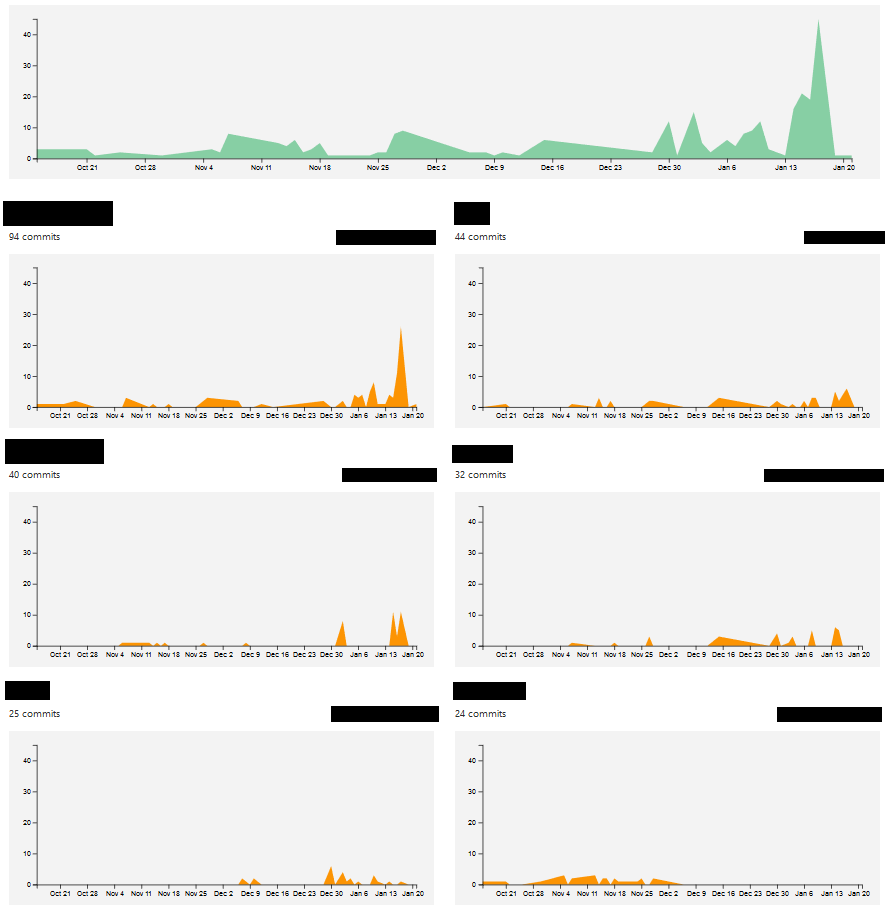
\includegraphics[scale=0.4]{slike/aktivnost.PNG} %veličina slike u odnosu na originalnu datoteku i pozicija slike
			\centering
			\caption{Primjer slike s potpisom}
			\label{fig:promjene}
		\end{figure}
		
		\begin{figure}[H]
			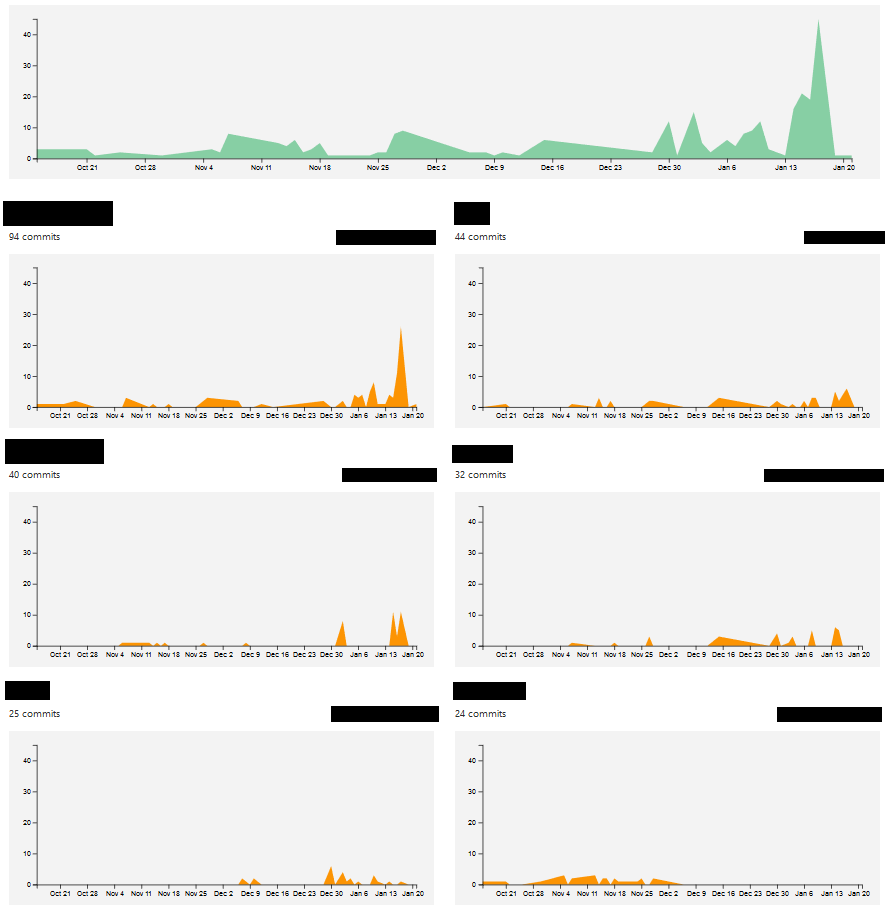
\includegraphics[width=\textwidth]{slike/aktivnost.PNG} %veličina u odnosu na širinu linije
			\caption{Primjer slike s potpisom 2}
			\label{fig:promjene2} %label mora biti drugaciji za svaku sliku
		\end{figure}
		
		Referenciranje slike \ref{fig:promjene2} u tekstu.
		
		\eject
		
	